\documentclass{standalone}
\usepackage{tikz}

\begin{document}

\tikzset{every picture/.style={line width=0.75pt}} %set default line width to 0.75pt        

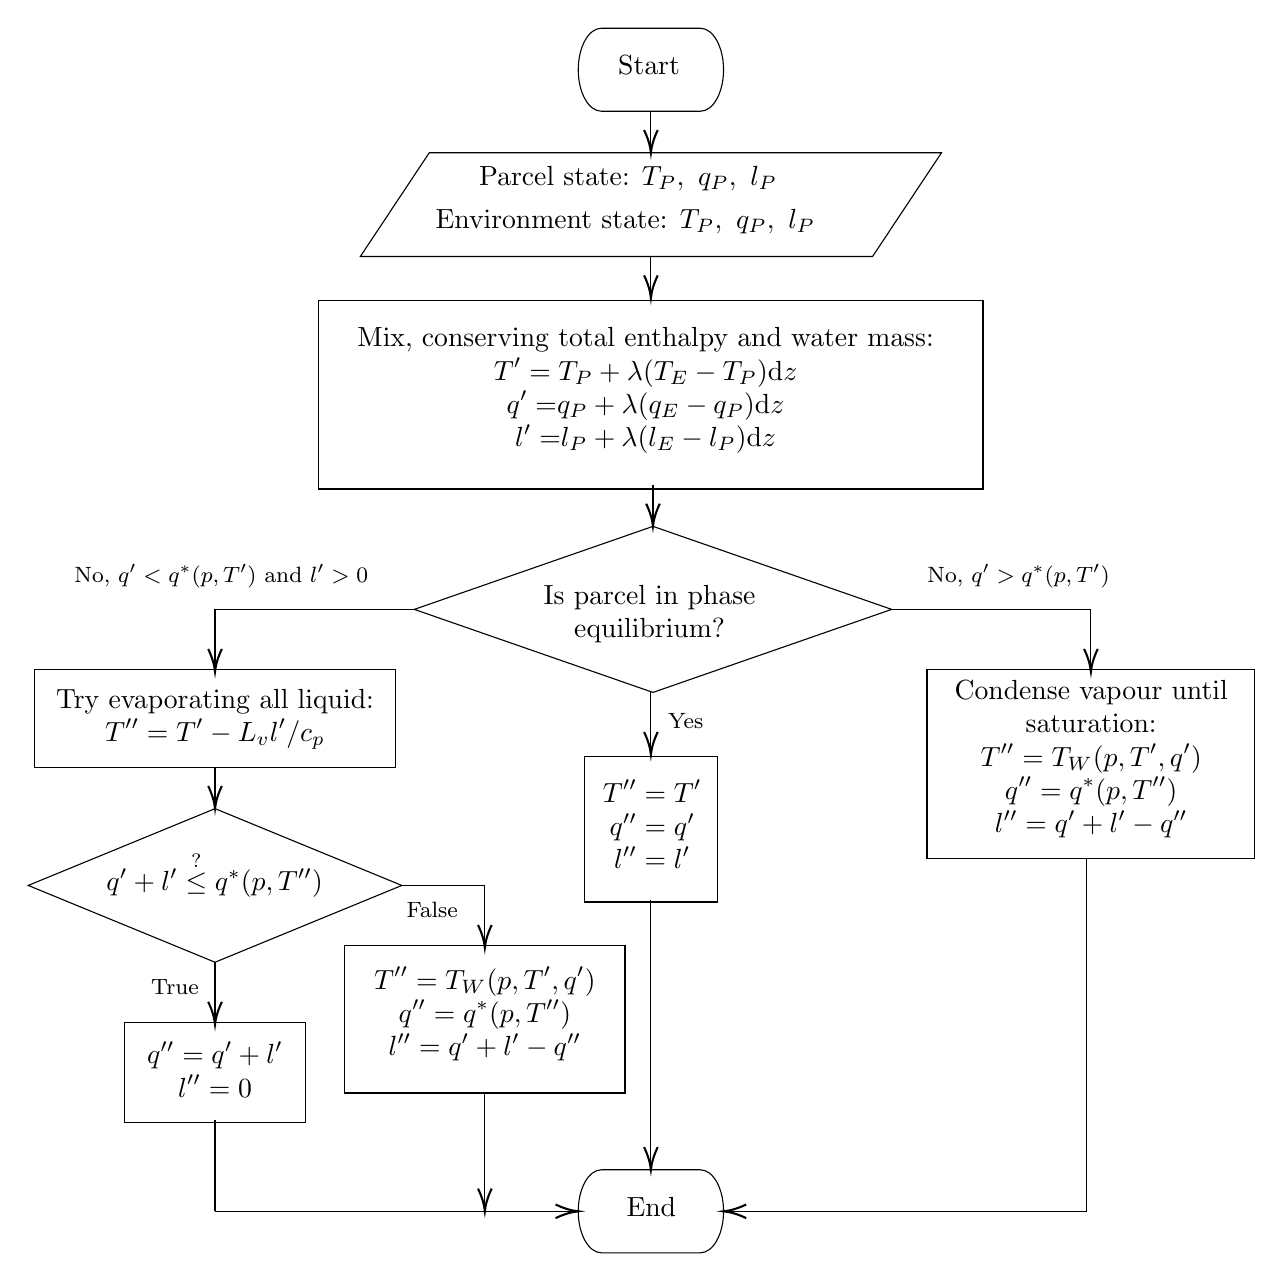
\begin{tikzpicture}[x=0.75pt,y=0.75pt,yscale=-1,xscale=1]
%uncomment if require: \path (0,673); %set diagram left start at 0, and has height of 673

%Flowchart: Terminator [id:dp03399036622468432] 
\draw   (296.2,60) -- (343.8,60) .. controls (349.99,60) and (355,68.95) .. (355,80) .. controls (355,91.05) and (349.99,100) .. (343.8,100) -- (296.2,100) .. controls (290.01,100) and (285,91.05) .. (285,80) .. controls (285,68.95) and (290.01,60) .. (296.2,60) -- cycle ;

%Shape: Parallelogram [id:dp67772339323324] 
\draw   (213.22,120) -- (460,120) -- (426.78,170) -- (180,170) -- cycle ;
%Flowchart: Decision [id:dp5791911401055645] 
\draw   (321,300) -- (436,340) -- (321,380) -- (206,340) -- cycle ;

%Straight Lines [id:da25008868194083167] 
\draw    (320,100) -- (320,118) ;
\draw [shift={(320,120)}, rotate = 270] [color={rgb, 255:red, 0; green, 0; blue, 0 }  ][line width=0.75]    (10.93,-3.29) .. controls (6.95,-1.4) and (3.31,-0.3) .. (0,0) .. controls (3.31,0.3) and (6.95,1.4) .. (10.93,3.29)   ;
%Straight Lines [id:da983740733769694] 
\draw    (320,170) -- (320,188) ;
\draw [shift={(320,190)}, rotate = 270] [color={rgb, 255:red, 0; green, 0; blue, 0 }  ][line width=0.75]    (10.93,-3.29) .. controls (6.95,-1.4) and (3.31,-0.3) .. (0,0) .. controls (3.31,0.3) and (6.95,1.4) .. (10.93,3.29)   ;
%Straight Lines [id:da6584022233120475] 
\draw    (321,280) -- (321,298) ;
\draw [shift={(321,300)}, rotate = 270] [color={rgb, 255:red, 0; green, 0; blue, 0 }  ][line width=0.75]    (10.93,-3.29) .. controls (6.95,-1.4) and (3.31,-0.3) .. (0,0) .. controls (3.31,0.3) and (6.95,1.4) .. (10.93,3.29)   ;
%Straight Lines [id:da9739098455781403] 
\draw    (110,340) -- (206,340) ;
%Straight Lines [id:da2743850670602297] 
\draw    (436,340) -- (532,340) ;
%Straight Lines [id:da12193385989550376] 
\draw    (110,340) -- (110,368) ;
\draw [shift={(110,370)}, rotate = 270] [color={rgb, 255:red, 0; green, 0; blue, 0 }  ][line width=0.75]    (10.93,-3.29) .. controls (6.95,-1.4) and (3.31,-0.3) .. (0,0) .. controls (3.31,0.3) and (6.95,1.4) .. (10.93,3.29)   ;
%Straight Lines [id:da18286409594266573] 
\draw    (532,340) -- (532,368) ;
\draw [shift={(532,370)}, rotate = 270] [color={rgb, 255:red, 0; green, 0; blue, 0 }  ][line width=0.75]    (10.93,-3.29) .. controls (6.95,-1.4) and (3.31,-0.3) .. (0,0) .. controls (3.31,0.3) and (6.95,1.4) .. (10.93,3.29)   ;
%Straight Lines [id:da021877348889204562] 
\draw    (320,380) -- (320,408) ;
\draw [shift={(320,410)}, rotate = 270] [color={rgb, 255:red, 0; green, 0; blue, 0 }  ][line width=0.75]    (10.93,-3.29) .. controls (6.95,-1.4) and (3.31,-0.3) .. (0,0) .. controls (3.31,0.3) and (6.95,1.4) .. (10.93,3.29)   ;
%Flowchart: Decision [id:dp2057314197294111] 
\draw   (110,436) -- (200,473) -- (110,510) -- (20,473) -- cycle ;

%Straight Lines [id:da40140575172712833] 
\draw    (110,416) -- (110,434) ;
\draw [shift={(110,436)}, rotate = 270] [color={rgb, 255:red, 0; green, 0; blue, 0 }  ][line width=0.75]    (10.93,-3.29) .. controls (6.95,-1.4) and (3.31,-0.3) .. (0,0) .. controls (3.31,0.3) and (6.95,1.4) .. (10.93,3.29)   ;
%Straight Lines [id:da4187788250058906] 
\draw    (110,510) -- (110,538) ;
\draw [shift={(110,540)}, rotate = 270] [color={rgb, 255:red, 0; green, 0; blue, 0 }  ][line width=0.75]    (10.93,-3.29) .. controls (6.95,-1.4) and (3.31,-0.3) .. (0,0) .. controls (3.31,0.3) and (6.95,1.4) .. (10.93,3.29)   ;
%Straight Lines [id:da9758455481631778] 
\draw    (200,473) -- (240,473) ;
%Straight Lines [id:da32213155759976364] 
\draw    (240,473) -- (240,501) ;
\draw [shift={(240,503)}, rotate = 270] [color={rgb, 255:red, 0; green, 0; blue, 0 }  ][line width=0.75]    (10.93,-3.29) .. controls (6.95,-1.4) and (3.31,-0.3) .. (0,0) .. controls (3.31,0.3) and (6.95,1.4) .. (10.93,3.29)   ;
%Flowchart: Terminator [id:dp6126624606056799] 
\draw   (296.2,610) -- (343.8,610) .. controls (349.99,610) and (355,618.95) .. (355,630) .. controls (355,641.05) and (349.99,650) .. (343.8,650) -- (296.2,650) .. controls (290.01,650) and (285,641.05) .. (285,630) .. controls (285,618.95) and (290.01,610) .. (296.2,610) -- cycle ;

%Straight Lines [id:da32092529474111675] 
\draw    (110,630) -- (283,630) ;
\draw [shift={(285,630)}, rotate = 180] [color={rgb, 255:red, 0; green, 0; blue, 0 }  ][line width=0.75]    (10.93,-3.29) .. controls (6.95,-1.4) and (3.31,-0.3) .. (0,0) .. controls (3.31,0.3) and (6.95,1.4) .. (10.93,3.29)   ;
%Straight Lines [id:da9514696204328044] 
\draw    (110,630) -- (110,586) ;
%Straight Lines [id:da9838563319346505] 
\draw    (240,628) -- (240,573) ;
\draw [shift={(240,630)}, rotate = 270] [color={rgb, 255:red, 0; green, 0; blue, 0 }  ][line width=0.75]    (10.93,-3.29) .. controls (6.95,-1.4) and (3.31,-0.3) .. (0,0) .. controls (3.31,0.3) and (6.95,1.4) .. (10.93,3.29)   ;
%Straight Lines [id:da03025058720776963] 
\draw    (320,480) -- (320,608) ;
\draw [shift={(320,610)}, rotate = 270] [color={rgb, 255:red, 0; green, 0; blue, 0 }  ][line width=0.75]    (10.93,-3.29) .. controls (6.95,-1.4) and (3.31,-0.3) .. (0,0) .. controls (3.31,0.3) and (6.95,1.4) .. (10.93,3.29)   ;
%Straight Lines [id:da8238743736461536] 
\draw    (530,630) -- (357,630) ;
\draw [shift={(355,630)}, rotate = 360] [color={rgb, 255:red, 0; green, 0; blue, 0 }  ][line width=0.75]    (10.93,-3.29) .. controls (6.95,-1.4) and (3.31,-0.3) .. (0,0) .. controls (3.31,0.3) and (6.95,1.4) .. (10.93,3.29)   ;
%Straight Lines [id:da4559101748513841] 
\draw    (530,630) -- (530,460) ;

% Text Node
\draw    (160,191) -- (480,191) -- (480,282) -- (160,282) -- cycle  ;
\draw (173,203) node [anchor=north west][inner sep=0.75pt]   [align=left] {\begin{minipage}[lt]{214.76pt}\setlength\topsep{0pt}
\begin{center}
Mix, conserving total enthalpy and water mass:\\$\displaystyle T'=T_{P} +\lambda ( T_{E} -T_{P})\mathrm{d} z$\\$\displaystyle q'=$$\displaystyle q_{P} +\lambda ( q_{E} -q_{P})\mathrm{d} z$\\$\displaystyle l'=$$\displaystyle l_{P} +\lambda ( l_{E} -l_{P})\mathrm{d} z$
\end{center}

\end{minipage}};
% Text Node
\draw (263,326.89) node [anchor=north west][inner sep=0.75pt]   [align=left] {\begin{minipage}[lt]{82.67pt}\setlength\topsep{0pt}
\begin{center}
Is parcel in phase\\equilibrium?
\end{center}

\end{minipage}};
% Text Node
\draw (303,72) node [anchor=north west][inner sep=0.75pt]   [align=left] {Start};
% Text Node
\draw (41,317) node [anchor=north west][inner sep=0.75pt]  [font=\footnotesize] [align=left] {No, $\displaystyle q'< q^{*}( p,T')$ and $\displaystyle l' >0$};
% Text Node
\draw (452,317) node [anchor=north west][inner sep=0.75pt]  [font=\footnotesize] [align=left] {No, $\displaystyle q' >q^{*}( p,T')$};
% Text Node
\draw (327,389) node [anchor=north west][inner sep=0.75pt]  [font=\footnotesize] [align=left] {Yes};
% Text Node
\draw    (453,369) -- (611,369) -- (611,460) -- (453,460) -- cycle  ;
\draw (461,373) node [anchor=north west][inner sep=0.75pt]   [align=left] {\begin{minipage}[lt]{104.79pt}\setlength\topsep{0pt}
\begin{center}
Condense vapour until\\saturation:\\$\displaystyle T''=T_{W}( p,T',q')$\\$\displaystyle q''=q^{*}( p,T'')$\\$\displaystyle l''=q'+l'-q''$
\end{center}

\end{minipage}};
% Text Node
\draw    (288,411) -- (352,411) -- (352,481) -- (288,481) -- cycle  ;
\draw (292,421) node [anchor=north west][inner sep=0.75pt]   [align=left] {\begin{minipage}[lt]{41.1pt}\setlength\topsep{0pt}
\begin{center}
$\displaystyle T''=T'$\\$\displaystyle q''=q'$\\$\displaystyle l''=l'$
\end{center}

\end{minipage}};
% Text Node
\draw    (23,369) -- (197,369) -- (197,416) -- (23,416) -- cycle  ;
\draw (110,377) node [anchor=north] [inner sep=0.75pt]   [align=left] {\begin{minipage}[lt]{115.74pt}\setlength\topsep{0pt}
\begin{center}
Try evaporating all liquid:\\$\displaystyle T''=T'-L_{v} l'/c_{p}$
\end{center}

\end{minipage}};
% Text Node
\draw (109.83,455.27) node [anchor=north] [inner sep=0.75pt]   [align=left] {\begin{minipage}[lt]{86.63pt}\setlength\topsep{0pt}
\begin{center}
$\displaystyle q'+l'\stackrel{?}{\leq } q^{*}( p,T'')$
\end{center}

\end{minipage}};
% Text Node
\draw (78,517) node [anchor=north west][inner sep=0.75pt]  [font=\footnotesize] [align=left] {True};
% Text Node
\draw    (66.5,539) -- (153.5,539) -- (153.5,587) -- (66.5,587) -- cycle  ;
\draw (110,547) node [anchor=north] [inner sep=0.75pt]   [align=left] {\begin{minipage}[lt]{56.42pt}\setlength\topsep{0pt}
\begin{center}
$\displaystyle q''=q'+l'$\\$\displaystyle l''=0$
\end{center}

\end{minipage}};
% Text Node
\draw (201,480) node [anchor=north west][inner sep=0.75pt]  [font=\footnotesize] [align=left] {False};
% Text Node
\draw    (172.5,502) -- (307.5,502) -- (307.5,573) -- (172.5,573) -- cycle  ;
\draw (240,511) node [anchor=north] [inner sep=0.75pt]   [align=left] {\begin{minipage}[lt]{89.21pt}\setlength\topsep{0pt}
\begin{center}
$\displaystyle T''=T_{W}( p,T',q')$\\$\displaystyle q''=q^{*}( p,T'')$\\$\displaystyle l''=q'+l'-q''$
\end{center}

\end{minipage}};
% Text Node
\draw (307,622) node [anchor=north west][inner sep=0.75pt]   [align=left] {End};
% Text Node
\draw (236,125.29) node [anchor=north west][inner sep=0.75pt]   [align=left] {Parcel state: $\displaystyle T_{P} ,\ q_{P} ,\ l_{P}$};
% Text Node
\draw (215,145.86) node [anchor=north west][inner sep=0.75pt]   [align=left] {Environment state: $\displaystyle T_{P} ,\ q_{P} ,\ l_{P}$};


\end{tikzpicture}

\end{document}